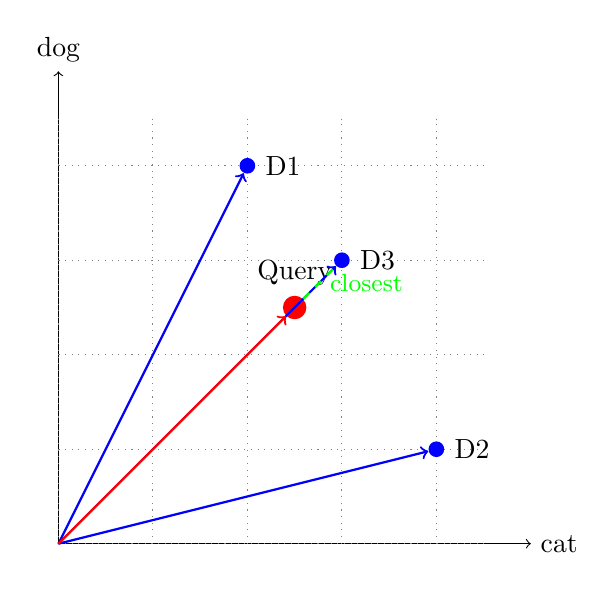
\begin{tikzpicture}[scale=1.2]
    % Axes
    \draw[->] (0,0) -- (5,0) node[right] {cat};
    \draw[->] (0,0) -- (0,5) node[above] {dog};
    
    % Grid
    \draw[gray, dotted] (0,0) grid (4.5,4.5);
    
    % Documents
    \node[circle, fill=blue, inner sep=2pt, label=right:D1] (d1) at (2,4) {};
    \node[circle, fill=blue, inner sep=2pt, label=right:D2] (d2) at (4,1) {};
    \node[circle, fill=blue, inner sep=2pt, label=right:D3] (d3) at (3,3) {};
    
    % Query
    \node[circle, fill=red, inner sep=3pt, label=above:Query] (q) at (2.5,2.5) {};
    
    % Vectors
    \draw[->, thick, blue] (0,0) -- (d1);
    \draw[->, thick, blue] (0,0) -- (d2);
    \draw[->, thick, blue] (0,0) -- (d3);
    \draw[->, thick, red] (0,0) -- (q);
    
    % Similarity illustration
    \draw[dashed, green, thick] (q) -- (d3) node[midway, right] {\small closest};
\end{tikzpicture}
